% tlpguide.tex
% v1.0, released 24 Mar 2021
% Copyright 2021 Cambridge University Press

\documentclass{tlp}

\usepackage{mathptmx}
\usepackage{amsmath, amssymb, amsfonts}
\usepackage{graphicx}
\usepackage{booktabs}
\usepackage{listings}
\usepackage{xcolor}
\usepackage{url}


\lstset{
  language=Prolog,                  % linguaggio simile ad ASP
  basicstyle=\ttfamily\small,      % font monospaziato piccolo
  numbers=left,                    % numero di riga
  numberstyle=\tiny\color{gray},   % stile dei numeri di riga
  stepnumber=1,                    % ogni riga è numerata
  numbersep=5pt,                   % distanza numeri dal codice
  backgroundcolor=\color{white},  % sfondo bianco
  showspaces=false,
  showstringspaces=false,
  showtabs=false,
  frame=single,                    % box attorno al codice
  rulecolor=\color{black},
  captionpos=b,                    % caption sotto
  breaklines=true,                 % va a capo automaticamente
  breakatwhitespace=true,
  tabsize=2,
  keywordstyle=\color{blue},
  commentstyle=\color{gray}\itshape,
  morecomment=[l]\%
}

\begin{document}



%\jnlPage{1}{8}
%\jnlDoiYr{2021}
%\doival{10.1017/xxxxx}

\title[An ASP-based Solution to the Medical Appointment Scheduling Problem]{An ASP-based Solution to the Medical Appointment Scheduling Problem}

\begin{authgrp}
\author{\sn{Vozna} \gn{Alina(1,2)}, 
\sn{Costantini} \gn{Stefania (1)}, \sn{Monaldini} \gn{Andrea (1,2)}, \sn{Pado} \gn{Dawid (1)}, \sn{Pitoni} \gn{Valentina (1)}}
\affiliation{(1) Department of Information Engineering, Computer Science and Mathematics,
University of L’Aquila,Italy, \\(2) University of Pisa, Largo B. Pontecorvo, Pisa,
56127, Italy}

\end{authgrp}



\maketitle

\begin{abstract}
This paper presents an Answer Set Programming (ASP)-based framework for medical appointment scheduling, aimed at improving efficiency, reducing administrative overhead, and enhancing patient-centered care. The framework personalizes scheduling for vulnerable populations by integrating Blueprint Personas. It ensures real-time availability updates, conflict-free assignments, and seamless interoperability with existing healthcare platforms by centralizing planning operations within an ASP logic model.

\end{abstract}

\begin{keywords}
Answer Set Programming, Healthcare, Logic Programming, Blueprint Personas, Preferences
\end{keywords}


\section{Introduction}
\label{introduction}

In the healthcare sector, effectively managing medical appointments is crucial to ensuring the efficient operation of healthcare facilities and enhancing patient experiences. An optimized scheduling system minimizes patient waiting times, reduces the occurrence of no-shows and last-minute cancellations, and ensures an equitable allocation of medical resources. The growing demand for healthcare services, driven by aging populations and an increase in chronic diseases, has further underscored the need for advanced scheduling solutions capable of handling multiple constraints simultaneously. In addition, appointment scheduling plays a crucial role in balancing patient access to care and healthcare resource optimization, yet traditional systems struggle to manage this balance effectively \citep{gupta2008appointment}.

Conventional scheduling methods, which typically depend on manual coordination or rule-based software, often face challenges in juggling competing priorities such as patient urgency, clinician availability, and resource allocation. Consequently, inefficiencies such as extended waiting periods, clinician fatigue, and suboptimal use of medical facilities occur frequently \citep{alrefaei2015modelling}. Moreover, rigid scheduling frameworks lack the flexibility to dynamically adjust to real-time variations in patient needs and staff availability, leading to suboptimal decision making and resource misallocation.

Consider, for instance, a patient with social anxiety who prefers early morning appointments in less crowded clinics. Assigning them to a midday slot in a busy urban center not only causes stress but also increases the likelihood of no-shows or cancellations. Often based on simple rule-based logic or first-come-first-served strategies, current systems rarely account for such nuanced preferences and constraints.

To address these challenges, this paper proposes an appointment scheduling system based on Answer Set Programming (ASP) \citep{baral2003knowledge,lifschitz2008handbook,costantini2010answer,lifschitz2019answer}, a declarative logic programming paradigm well suited for complex decision-making under multiple constraints.

By combining ASP’s expressiveness with patient-centered modeling, the system ensures real-time adaptability, constraint satisfaction, and ethically grounded resource allocation. The solution automatically filters out invalid appointment options (e.g., inaccessible clinics for disabled patients or incompatible time slots). It optimizes scheduling according to criteria such as urgency, clinician availability, patient preferences, and budget constraints.

A crucial aspect of the proposed patient-centered scheduling is the integration of Blueprint Personas, which provide structured, persona-driven models that capture patient needs, preferences, and behaviors \citep{monaldini2024blueprint}. Blueprint Personas, which were initially created as part of digital health transformation projects, are a tool to create individualized healthcare experiences by coordinating appointment scheduling with the conditions, accessibility requirements, and lifestyle limitations of each patient. Healthcare providers can improve adherence to medical visits, ensure more equitable access to care, and develop adaptive scheduling policies that prioritize vulnerable groups by integrating Blueprint Personas into scheduling frameworks. 


The inherent ability of ASP to handle dynamic constraints makes it particularly effective in real-world healthcare scenarios where last-minute cancellations, emergency cases, and fluctuating resource availability must be seamlessly incorporated into the scheduling process. The proposed approach is evaluated against traditional scheduling methodologies to demonstrate its superiority in minimizing waiting times, enhancing resource utilization, and improving overall patient satisfaction.

\paragraph{Methodological Contribution.}
While several scheduling systems rely on ad hoc or heuristic-driven methods, our contribution lies in demonstrating how a fully declarative, patient-centered scheduling framework can be modeled systematically using ASP. We highlight the integration of complex multi-objective optimization, including patient sensory preferences, accessibility requirements, and real-time constraints, in a unified logic-based system. Moreover, we propose a modular modeling approach, enabling easy generalization to other domains such as workforce scheduling or education timetabling.

The paper is structured as follows: Section~\ref{related} discusses background and related work in the scheduling of medical appointments and ASP-based optimization; Section~\ref{problem-description} presents the formulation of the problem, detailing the constraints and objectives of the scheduling model; Section~\ref{architecture} describes the ASP-based system architecture and implementation; Section~\ref{experiments} provides an empirical evaluation of the approach, comparing its performance with conventional scheduling methods; finally, in Section~\ref{conclusion} we conclude and discuss future research directions.

\section{Related work}
\label{related}

Appointment scheduling has been widely studied using queueing theory, integer programming, and simulation models to address variability in service times, patient no-shows, and resource limitations (Gupta and Denton, 2008). More recent studies have extended this perspective by incorporating decision-support tools to optimize scheduling in outpatient clinics \citep{niu2023review}.

Optimization techniques, such as Mixed-Integer Linear Programming (MILP), ASP, and metaheuristic algorithms, have been widely applied to address scheduling challenges. Their effectiveness for optimizing overbooking strategies to balance patient access and hospital resource utilization has been demonstrated by Stochastic programming methods \citep{kuo2020medical}. Similarly, heuristic approaches, such as Fuzzy Ant Lion Optimization (FALO), have been applied to improve fairness in scheduling, significantly reducing patient waiting times while maintaining high resource efficiency \citep{ala2022appointment}. Discrete Event Simulation (DES), integrated with patient behavior modeling and genetic algorithms, has also enhanced scheduling by accounting for preferences, cancellations, and patient flow \citep{fan2021outpatient}.

%Multi-objective metaheuristics such as the Whale Optimization Algorithm (WOA) and NSGA-II have balanced resource allocation and patient satisfaction more effectively than traditional FCFS approaches \citep{ala2021optimization}. 
ASP has proven effective in resource-constrained domains, such as operating room \citep{dodaro2024operating} and nurse scheduling \citep{alviano2019nurse}, offering flexibility and efficiency compared to SAT and other methods.

Recent improvements in artificial intelligence (AI) have enabled machine learning and reinforcement learning-based appointment scheduling. Studies have integrated AI models with historical patient behavior data to predict and dynamically update scheduling \citep{ala2022appointment2}.

AI-driven methods, including reinforcement learning and deep learning, have emerged as powerful tools for improving appointment scheduling. Metaheuristic algorithms, such as genetic algorithms and neural networks, have been used to improve resource utilization by minimizing patient waiting times \citep{niu2023review}. Hybrid models have been developed for complex scenarios like MRI scheduling, using two-stage stochastic programming with evolutionary algorithms to manage uncertainty and improve utilization \citep{qiu2019mri}. Decentralized approaches have modeled scheduling as a Distributed Constraint Optimization Problem (DCOP), framing it as a negotiation process between agents \citep{hannebauer2001distributed}.

Despite the advances, a persistent gap remains between theoretical models and real-world healthcare constraints. Practical factors such as unpredictable patient behavior, clinician workload, and process complexity are often overlooked \citep{kuiper2021problem}. 

\paragraph{Positioning of Our Work.}
Unlike optimization methods based on heuristics, machine learning, or stochastic programming, our ASP-based framework guarantees strict satisfaction of hard constraints, full explainability of decisions, and easy adaptability to evolving requirements. Furthermore, while several prior works address resource scheduling, few integrate patient-centric factors such as sensory preferences, accessibility needs, and financial constraints holistically. Our work bridges this gap by proposing a patient-centered, constraint-driven, and ethically grounded scheduling solution, leveraging the declarative modeling power of ASP.




\vspace{-0.5cm}
\section{Problem Description and Formalization}
\label{problem-description}

Effectively managing medical appointments is a multidimensional challenge that involves clinical urgency, resource availability, patient preferences, and logistical constraints; traditional approaches often fail to reconcile these factors simultaneously.

To address this, we formulate the appointment scheduling task as a multi-objective constrained optimization problem, solved using ASP. The declarative nature of ASP enables a concise representation of domain constraints and an automated search for feasible and optimal solutions.

The scheduling problem is modeled as follows:
\begin{itemize}
    \item \textbf{Clinics:} Each clinic has a set of available time slots and a limited budget.
    \item \textbf{Doctors:} Each doctor is assigned to a clinic and can only manage a certain number of patients per day.
    \item \textbf{Patients:} Each patient has a priority (high, medium, low), preferred clinics, and possibly sensory preferences.
    \item \textbf{Slots:} Each slot represents a fixed time at which a visit can be scheduled.
\end{itemize}
The aim is to assign each patient to one or more appointment slots so that all hard constraints are satisfied and the overall utility is maximized. The objectives include:
\begin{enumerate}
    \item Minimizing patient waiting times by prioritizing early scheduling.
    \item Ensure equitable workload allocation across all physicians.
    \item Maximizing adherence to patient preferences, such as preferred time slots or doctors.
    \item Optimize resource allocation by avoiding overbooking and idle time.
\end{enumerate}

The ASP model treats appointment scheduling as a Constraint Satisfaction Problem (CSP) augmented with optimization objectives: hard constraints eliminate invalid assignments, while soft constraints guide the selection of optimal configurations.

\subsection{Formal Problem Statement}
\label{sec:formalproblem}

We formalize the medical appointment scheduling task as a constrained optimization problem defined as follows.

\paragraph{Given:}
\begin{itemize}
    \item A set $P$ of patients, each characterized by a priority level $\text{priority}(p) \in \{\text{high}, \text{medium}, \text{low}\}$, clinical needs, and a set of preferences over time slots, doctors, clinics, and environmental conditions.
    \item A set $D$ of doctors, each with specific expertise and capacity constraints.
    \item A set $C$ of clinics, each with available time slots, accessibility features, and budgetary constraints.
    \item A set $S$ of available time slots, distributed among clinics and doctors.
\end{itemize}

\paragraph{Constraints:}
\begin{itemize}
    \item Each patient must be assigned the required number of appointments matching their treatment plan.
    \item Assignments must respect hard constraints: accessibility requirements, clinic budgets, visit compatibility, and clinician availability.
    \item No double-booking is permitted for the same doctor, clinic, and time slot.
\end{itemize}

\paragraph{Objective:}
Find an assignment function $f : P \to (D \times C \times S)$ that:
\begin{enumerate}
    \item Minimizes overall patient waiting times.
    \item Maximizes satisfaction of patient preferences (preferred clinics, doctors, time windows, environmental conditions).
    \item Ensures equitable workload distribution among doctors.
    \item Minimizes total operational penalties (sensory mismatches, resource overuse).
\end{enumerate}

This formalization naturally maps to an Answer Set Programming (ASP) model, where feasible assignments correspond to answer sets satisfying the constraints and optimization goals.


\subsection{User Modeling and Personas}
Effective appointment scheduling requires more than managing clinical data; it demands understanding patients as individuals with unique needs, preferences, and constraints. For this reason, we adopt \textbf{Blueprint Personas}, structured archetypes originally developed within European digital health initiatives (EIP on AHA) \citep{EIP_AHA}, which encapsulate real-world profiles combining clinical, social, cognitive, and behavioral attributes. Blueprint Personas enable a layer of abstraction between raw data and decision logic, allowing our system to reason over individualized scheduling needs in a flexible and human-centered way.

\medskip
\noindent\textbf{Patient personas}: 
Each patient persona is a combination of health status, socio-environmental factors, and digital literacy; this model allows the system to reason over complex, individualized scheduling needs. There are three different levels of patient complexity:
\begin{itemize}
    \item \textbf{Generally healthy individuals}: prefer convenient scheduling (e.g., early mornings, nearby clinics) but have no strict clinical constraints. %Example: Lucia De Santis, 29, a vegetarian with lactose intolerance, works full-time and prefers lunchtime or evening virtual visits with a nutritionist. While she doesn’t face urgent clinical needs, she requires time-slot compatibility with work and dietary-specific care.    
    \item \textbf{People with chronic conditions}: require regular follow-ups, budget-sensitive allocation, and minimal waiting times; the scheduling must comply with multi-visit intervals and cost limits. %Example: Giovanni Rinaldi, 78, lives alone and is monitored remotely for diabetes and hypertension. He prefers morning appointments with his geriatrician or MMG.   
    \item \textbf{Patients with complex needs}: may express sensory sensitivities (e.g., noise, lighting), require accessible facilities, or depend on caregivers for travel; the system must respect personalized preferences and environmental constraints. %Anna Ricci, 35, suffers from social anxiety and mild agoraphobia. She avoids crowded waiting areas and prefers late or early slots.
 \end{itemize}   
 
Key personal data identify patients and can express preferences for clinics, time slots, sensory conditions, and doctors. Travel distance is also considered, with a fixed value of 0 for Home Care and Telemedicine.

\begin{lstlisting}[language=Prolog, caption=Patient Profile with Preferences and Constraints]
patient(p1, "Mario", "Rossi", "L'Aquila"). disabled(p1).
preference(p1, c3).
sensory_preference(p1, "noise").
doctor_preference(p1, "GP", "chronic_diseases", 10).
appointment_preference(p1, c3, 1850, 2000).
distance(p1, c3, 15).
\end{lstlisting}

\noindent
\textbf{Clinician Personas}: Equally important is the modeling of medical professionals; each clinician's persona describes, at least, their specialty, technological commitment, and operational challenges. This allows the system to anticipate realistic workload constraints and optimize care coordination. 

For each available clinic, the \textbf{visit\_type} represents the characteristics of the treatments offered in the clinics. Each visit is identified by: name, cost, and classification indicating its chronicity (0 = non-chronic, 1 = chronic), and the need for an in-person visit. Some visits require several sessions, with minimum and maximum intervals that must be followed:
\begin{lstlisting}[language=Prolog, caption=Visit Type Definition and Constraints]
visit_type(v1, "Cardiology", "Heart Attack", 0, 0, 0).
visit_cost(v1, 1000).
required_sessions(v1, 2).
session_interval(v1, 14, 28).
\end{lstlisting}

Clinic availability is defined by Unix timestamps, marking specific times for medical appointments. Each patient request includes an urgency level (1–3) and a preferred interval between sessions, thus enabling optimal scheduling based on personal needs and budget.

\begin{lstlisting}[language=Prolog, caption=Patient Needs Preferences and Clinic Availability]
patient_interval(p1, v1, 21, 28).         
need(p1, v1, 3).                           
availability(c1, v1, 1727308800).         
\end{lstlisting}


%\subsection{Combined Scenario-Based Evaluation}

%Dr. Marco Bianchi is a seasoned general practitioner with over 25 years of experience. 
%He works in a private medical office and collaborates with the local health authority (ASL). 
%He regularly uses electronic health records (EHR) and telemedicine solutions. 
%Despite embracing digital tools, his main challenge is managing a high volume of patients, which limits the time available per visit.

%\textbf{Technological context:} EHR systems, remote monitoring tools.\\
%\textbf{Key expectations:} 
%\begin{itemize}
   % \item An intelligent appointment scheduling assistant,
   % \item Reduction of administrative load,
    %\item Smart notification and reminder system.
%\end{itemize}




%These personas are directly mapped to model parameters in the ASP encoding:

%Sensory preferences → \texttt{sensory\_preference(Patient, Type)}

%Clinical urgency → \texttt{clinical\_urgency(Patient, Visit, Urgency)}

%Budget sensitivity → \texttt{budget(Clinic, Budget) + visit\_cost(...)}

%Multi-session care → \texttt{session\_required(...) + session\_interval(...)}

%Accessibility → \texttt{accessible(Clinic)}

This modeling enables the system to reason over patient-specific constraints and ensures that solutions are medically appropriate and patient-centered. The personas also support scenario-based validation: simulated patients can be run through the solver to assess how well the system accommodates edge cases and vulnerable users.

\vspace{-0.5cm}
\subsection{Rules of inference}
Inference rules in the ASP-based model derive intermediate knowledge from base facts, enhancing optimization beyond simple constraint filtering. Patient preferences, such as favorite clinics, are translated into weighted parameters that positively influence their assignment during minimization.
\begin{lstlisting}[language=Prolog, caption=Effect of Clinic Preference on Patient Assignment]
clinic_preference_effect(Patient, Clinic, 1) :-
    preference(Patient, Clinic).
clinic_preference_effect(Patient, Clinic, 0) :- not
    preference(Patient, Clinic).
\end{lstlisting}

The \textbf{chronics\_cost} is the total cost of each clinic for chronic visits, which is calculated by adding up the costs of each appointment that is associated with chronic visits. This value is useful in order to assess the respect of the budget available for
each clinic:
\begin{lstlisting}[language=Prolog, caption=Calculation of Total Cost for Chronic Patients]
chronics_cost(Clinic, TotalCost) :- clinic(Clinica _),
    TotalCost = #sum {
    Cost : appointment(Patient, Clinic, Visit, _),
    visit_type(Visit, _, _, 1), visit-cost(Visit, Cost)
    }.
\end{lstlisting}

The  \textbf{effect\_doctor\_preference} checks whether a doctor meets the patient's expressed preferences: returns 1 if the doctor matches the specialization and required experience, 0 otherwise. This value can guide the assignment process in the optimization function.

\begin{lstlisting}[language=Prolog, caption=Effect of Patient Preference on Doctor Assignment]
doctor_preference_effect(Patient, Doctor, 1) :-
    patient(Patient, _, _, _), 
    doctor(Doctor, _, _, _, _, Type),
    doctor_experience(Doctor, Specialization, YearsExperience),
    doctor_preference(Patient, Type, Specialization, RequiredYears),
    YearsExperience >= RequiredYears.
doctor_preference_effect(Patient, Doctor, 0) :-
    patient(Patient, _, _, _), 
    doctor(Doctor, _, _, _, _, Type),
    doctor_experience(Doctor, Specialization, _),
    not doctor_preference(Patient, Type, Specialization, _).
doctor_preference_effect(Patient, Doctor, 0) :-
    patient(Patient, _, _, _), 
    doctor(Doctor, _, _, _, _, Type),
    doctor_experience(Doctor, Specialization, YearsExperience),
    doctor_preference(Patient, Type, Specialization, RequiredYears),
    YearsExperience < RequiredYears.
\end{lstlisting}

The \textbf{effect\_appointment\_preference} determines whether a given appointment time aligns with a patient's preferred time range: returns 1 if the time falls within the specified range (Start to End), and 0 otherwise.
The time is transformed into a weighted score using hours and minutes to allow comparison with the preference interval; this value can be used in optimization to prioritize preferred time slots.

\begin{lstlisting}[language=Prolog, caption=Effect of Time Preference on Appointment Scheduling]
appointment_preference_effect(Patient, Time, Clinic, 1) :-
    patient(Patient, _, _, _), 
    clinic(Clinic, _),
    availability(Clinic, _, _, Time),
    appointment_preference(Patient, _, Start, End),
    X = (((Time \ 86400) * 3600) * 100) + (((Time \ 3600) / 60) / 3) * 5,
    X <= End, X >= Start.
appointment_preference_effect(Patient, Time, Clinic, 0) :-
    patient(Patient, _, _, _), 
    clinic(Clinic, _),
    availability(Clinic, _, _, Time),
    appointment_preference(Patient, _, Start, End),
    X = (((Time \ 86400) * 3600) * 100) + (((Time \ 3600) / 60) / 3) * 5,
    X > End.
appointment_preference_effect(Patient, Time, Clinic, 0) :-
    patient(Patient, _, _, _), 
    clinic(Clinic, _),
    availability(Clinic, _, _, Time),
    appointment_preference(Patient, _, Start, End),
    X = (((Time \ 86400) * 3600) * 100) + (((Time \ 3600) / 60) / 3) * 5,
    X < Start.
\end{lstlisting}


Finally, there are rules for evaluating sensory penalties. These rules are useful in determining the gap between the environmental conditions of the clinic and the patient’s expressed preferences. The penalty becomes void when the patient in question has not expressed any preference:
\begin{lstlisting}[language=Prolog, caption=Sensory Penalty Based on Environmental Conditions]
sensory_penalty(Patient, Clinic, Time, Level):-
    sensory_preference(Patient, Type),
    environmental_condition(Clinic, Type, Level, Start, End),
    Time >= Start, Time <= End.
sensory_penality(Patient, Clinic, Time, 0):- not
    sensory_preference(Patient, _).
\end{lstlisting}
%Below is an example of how this information is encoded in ASP:

%\begin{verbatim}
%clinic(c1, "Clinic A").
%budget(c1, 50000).
%accessible(c1).

%patient(p1, "Mario", "Rossi").
%preference(p1, c1).
%sensory_preference(p1, "noise").
%distance(p1, c1, 15).

%visit_type(v1, "Cardiology", "Heart Attack", 0).
%visit_cost(v1, 1000).
%required_sessions(v1, 2).
%session_interval(v1, 14, 28).

%availability(c1, v1, 1727308800).
%need(p1, v1, 3).
%\end{verbatim}
\vspace{-0.35cm}
\subsection{Constraints}

Constraints define the logical rules that each solution generated by the ASP model must comply with. They ensure that appointments are allocated in accordance with clinical, personal, and logistical requirements. 

First, each patient must be assigned exactly the number of appointments required for each treatment, according to their specific medical condition. This guarantees that treatments involving multiple sessions are correctly distributed across available time slots.

\begin{lstlisting}[language=Prolog, caption=Choice Rule for Appointment Allocation Based on Patient Needs]
Sessions{ appointment(Patient, Clinic, Doctor,  Visit, Time) : 
            availability(Clinic, DOctor, Visit, Time) }Sessions :- 
need(Patient, Visit, _), required_sessions(Visit, Sessions).
\end{lstlisting}


Moreover, to avoid scheduling conflicts, two patients can not be assigned the same clinic, visit type, and time slot simultaneously.

\begin{lstlisting}[language=Prolog, caption=Constraint Preventing Double Booking of the Same Slot]
:- appointment(P1, Clinic, Doctor, Visit, Time), appointment(P2, Clinic, Doctor, Visit, Time), P1 != P2.
\end{lstlisting}

Priority is also given to patients with high urgency, who must be scheduled in earlier slots, within a predefined temporal threshold.

\begin{lstlisting}[language=Prolog, caption=Constraint to Prioritize Urgent Visits]
:- needs(P1, Visit, Urg1), needs(P2, Visit, Urg2),
   Urg1 > Urg2, appointment(P1, Clinic, Doctor, Visit, Time1),
   appointment(P2, Clinic, Doctor, Visit, Time2),
   Time1 > Time2.
\end{lstlisting}


Accessibility needs are also addressed: patients with disabilities must only be assigned to clinics explicitly marked as accessible.

\begin{lstlisting}[language=Prolog, caption=Constraint Preventing Assignment to Inaccessible Clinics]
:- disabled(Patient), appointment(Patient, Clinic, _, _,_), not accessible(Clinic).
\end{lstlisting}

The model also respects the financial constraints of each clinic; the cumulative cost of scheduled chronic care appointments must not exceed the clinic’s allocated budget.

\begin{lstlisting}[language=Prolog, caption=Constraint to Respect Clinic Budget Limits]
:- chronic_cost(Clinic, TotalCost),
   budget(Clinic, Budget), TotalCost > Budget.
\end{lstlisting}

Some visits can occur via telemedicine or home care, but others require a doctor’s physical presence and must be on-site; this constraint prevents assigning visits to incompatible clinic types.

\begin{lstlisting}[language=Prolog, caption=Constraints for Incompatible Visit Types and Clinic Modes]
:- appointment(Patient, Clinic, Doctor, Visit, Time),
   visit_type(Visit, _, _, _, 1, _),
   clinic(Clinic, "Home Care").
:- appointment(Patient, Clinic, Doctor, Visit, Time),
   visit_type(Visit, _, _, _, 1, _),
   clinic(Clinic, "Telemedicine").
:- appointment(Patient, Clinic, Doctor, Visit, Time),
   visit_type(Visit, _, _, _, _, 1),
   clinic(Clinic, "Telemedicine").
\end{lstlisting}


\section{System Architecture}
\label{architecture}

The system is implemented as a set of loosely coupled microservices that are 
organized to manage appointment requests and generate optimal schedules based on ASP logic. The system is structured in three main layers: User Interface, Business Logic, and Data Management, to ensure scalability, maintainability, and integration with existing healthcare infrastructures.

The \textbf{User Layer} includes both web interfaces (e.g., browser) and IoT devices, which may trigger appointment requests automatically based on health parameter thresholds.

The \textbf{Business Logic Layer} consists of two Flask-based microservices \citep{newman2021building}:
\begin{itemize}
    \item MS1: handles incoming API requests, user authentication (via JWT tokens \citep{haekal2016token}), and formats the data into ASP facts.
    \item MS2: collects facts into a batch queue and, every 60 seconds, compiles them into a complete ASP program; this program is solved using Clingo \citep{gebser2014clingo}.
\end{itemize}

The \textbf{Data Layer} relies on a MySQL database, which maintains key information such as patient preferences, clinic features, appointment availability, environmental conditions, and budget constraints. All data interactions follow the ACID principles.

The system exposes several REST APIs for backend interaction; these include endpoints to submit appointment requests, check the status of ongoing bookings, and view up-to-date availability for each clinic. Asynchronous threading prevents overload during peak times, offering immediate user feedback and delayed result delivery.

Thanks to its layered architecture, centralized constraint management via ASP, and smooth integration with the Python backend, the system demonstrates effectiveness in handling complex scheduling scenarios. Moreover, the microservice-based structure allows individual components (e.g., solver, user interface, or database) to be updated or extended independently, without compromising the entire system.
The full source code is publicly available online \footnote{ \url{https://github.com/DawidPado/An-ASP-based-Solution-to-the-Medical-Appointment-Scheduling-Problem/tree/main}}.

%\begin{figure}[h!]
%\centering
%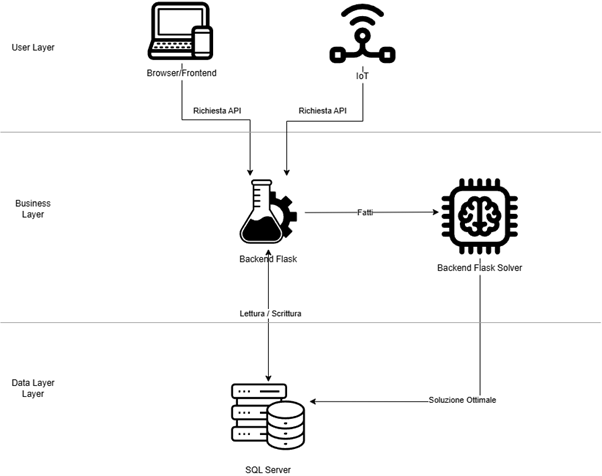
\includegraphics[width=0.5\textwidth]{architecture_en_base.png}
%\caption{Architecture of the ASP-based appointment scheduling system. }
%\label{fig:asp_architecture}
%\end{figure}

%The overall system architecture is illustrated in Figure~\ref{fig:asp_architecture}. It shows the flow of data from the user interface layer, through business logic, down to the database layer. The microservice design enables independent scaling and integration with external healthcare systems.




%Efficient scheduling of medical appointments requires handling multiple constraints simultaneously, including patient priorities, clinic availability, accessibility, individual preferences, and budget limits. Traditional systems, such as the Italian CUP (Centro Unico di Prenotazione) \citep{ministero2009cup} %l'ho buttata lì così ma serve un'introduzione are based on simple availability matching and lack the flexibility to handle complex constraints or rescheduling. This results in long waiting times, poor patient satisfaction, and suboptimal resource usage. To overcome these limitations, we propose a system that adopts a constraint-based, declarative approach using ASP. This approach enables the encoding of complex rules while allowing the system to automatically eliminate invalid solutions and identify optimal ones.

%The key principles guiding the system design are:
%\begin{itemize}
   % \item \textbf{Flexibility and expressiveness}: ASP allows a straightforward yet powerful representation of constraints, preferences, and objectives.
   % \item \textbf{Modularity}: Each component—data collection, logic encoding, and solving—is clearly separated, allowing adaptability and scalability.
  %  \item \textbf{Optimization-first logic}: Unlike greedy or heuristic methods, ASP guarantees that all constraints are satisfied before evaluating the objective function.
%\end{itemize}

%The system models the scheduling problem as a multi-criteria optimization task, considering:
%\begin{itemize}
 % \renewcommand\labelitemi{-}
  %\item Clinical priority (e.g., chronic or urgent conditions)
 % \item Time-based and sensory preferences
 % \item Accessibility requirements
 % \item Geographic distance to clinics
 % \item Budget constraints for chronic patients
 % \item Session continuity and multi-visit intervals
%\end{itemize}


%\subsection{Comparison with Alternative Approaches}
%Conventional systems such as CUP allocate appointments on a first-available basis, with limited regard for urgency, preferences, or follow-up logic. These systems require manual intervention in case of cancellations or changes, reducing overall efficiency.

%Alternative algorithmic approaches include a) Greedy heuristics \citep{branke2015automated}, which prioritize speed over constraint satisfaction, often leading to suboptimal results in complex scheduling scenarios and b) Linear Programming (LP) and Integer Programming, which require linear formulations and struggle with non-linear constraints like sensory compatibility or multi-slot dependencies.

%Compared to these, ASP offers a distinct advantage: 1) it declaratively encodes all constraints, ensuring only valid solutions are considered; 2) it allows for fine-grained control over optimization goals, including patient satisfaction factors; 3) it supports dynamic updates and fast re-solving, useful in clinical contexts where conditions can change rapidly.



%\subsection{ASP Encoding for Scheduling Optimization}
\vspace{-0.5cm}
\section{Experimental Evaluation}
\label{experiments}

To illustrate the flexibility and robustness of the proposed ASP-based scheduling framework, we present three realistic scheduling scenarios inspired by real-world medical scheduling needs. All tests were executed using Clingo 5.7.0 \footnote{\url{https://github.com/potassco/clingo/releases/tag/v5.7.0}}. The experiments demonstrate the system's ability to handle various constraints, from accessibility and urgency to sensory preferences and patient prioritization.

\subsection{Scenario 1: High-Priority Patient with Accessibility Requirements}
In this first scenario, a patient with a disability and a high-priority medical need requires a cardiology appointment. The patient, p1, must be scheduled for a visit type v1 (e.g., cardiology consultation) with urgency level 3. Due to the patient's condition, the appointment must be assigned only to clinics that are physically accessible. Listing~\ref{lst:scenario1} summarizes the key ASP facts for Scenario 1 in compressed form.


\begin{lstlisting}[language=Prolog,caption={ASP facts for Scenario 1 – High-priority disabled patient},label={lst:scenario1}]
% Scenario 1: High-priority disabled patient (compressed facts)
doctor(m1, "Marco", "Bianchi", 52, "L'Aquila", "GP").
patient(p1, "Mario", "Rossi"). disabled(p1).
clinic(c3, "Clinic A"). ... clinic(c5, "Clinic C").
accessible(c3). accessible(c5).
distance(p1, c3, 15). distance(p1, c4, 5). distance(p1, c5, 20).
visit_type(v1, "Cardiology", "Hypertension", 0, 1, 1). need(p1, v1, 3).
availability(c3, m1, v1, 1727308800). availability(c4, m1, v1, 1727481600).
availability(c5, m1, v1, 1727308800).
\end{lstlisting}
To ensure that the patient is only assigned to an accessible clinic, the following constraint has been introduced:

\begin{lstlisting}[language=Prolog, caption={Accessibility constraint for disabled patients}]
:- disable(Patient), appointment(Patient, Clinic, _, _,_),
    not accessibile(Clinic).
\end{lstlisting}


\textbf{Outcome:} The patient was correctly assigned to the nearest accessible clinic with the earliest available slot. All constraints (accessibility, urgency, distance) were satisfied. \textbf{Computation time:} 0.036s \textbf{Optimality:} Yes

\vspace{-0.5cm}
\subsection{Scenario 2 – Sensory Preferences}

A patient requests an orthopedic visit, expressing a preference for \textbf{bright environments}. The system must choose a clinic with suitable environmental conditions (light), and possibly sacrifice distance to respect sensory preferences.

\begin{lstlisting}[language=Prolog,caption={ASP facts for Scenario 2 – Sensory preference for brightness},label={lst:scenario2}]
% Patient and sensory preference
patient(p2, "Giulia", "Bianchi"). sensory_preference(p2, "light").
% Clinics and environmental conditions
clinic(c3, "Clinic A"). clinic(c4, "Clinic B").
environment_condition(c1, "light", 3, 1727480000, 1727489000).
environment_condition(c2, "light", 1, 1727480000, 1727489000).
distance(p2, c3, 10). distance(p2, c4, 25).
% Type of visit requested
visit_type(v2, "Orthopedics", "Kyphosis", 0, 1, 1).
visit_cost(v2, 1500). needs(p2, v2, 2).
% Slot availability
availability(c3, m1, v2, 1727481600). % 28.09.2024, 12:00
%...
\end{lstlisting}
To respect the patient’s sensory preferences, the model includes the following rule for calculating sensory penalties:
\begin{lstlisting}[language=Prolog, caption={Evaluation of sensory penalty based on clinic environment}]
sensory_penalty(Patient, Clinic, Time, Level):-
    sensory_penalty(Patient, Type),
    condizione_ambientale(Clinic, Type, Level, Start, End),
    Time >= Start, Time <= End.
sensory_penalty(Patient, Clinic, Time, 0) :- not
    sensory_penalty(Patient, _).
\end{lstlisting}

\textbf{Outcome:} The patient was assigned to a more distant clinic that satisfies her sensory preference (low lighting penalty). \textbf{Sensory penalty:} 0 \textbf{Computation time:} 0.017s \textbf{Optimality:} Yes

\vspace{-0.45cm}
\subsection{Scenario 3 – Group Prioritization}

Five patients request a cardiology visit at the same clinic. They differ in: \textbf{Urgency level}, \textbf{Preferences} (clinic, sensory), \textbf{Distance from the clinic}.
The model must prioritize based on urgency while minimizing penalties.
\begin{lstlisting}[language=Prolog,caption={ASP facts for Scenario 3 – Prioritization of 5 patients with limited slots},label={lst:scenario3}]
% Patients and urgency levels
patient(p1, "Mario", "Rossi"). needs(p1, v1, 3). % High urgency
patient(p2, "Giulia", "Bianchi"). needs(p2, v1, 2). % Medium 
%...
preference(p3, c3). preference(p3, c5).
% Distances from clinic
distance(p1, c3, 10). distance(p2, c3, 15).
%...
%Sensosy penalties
sensory_preference(p2, "light"). sensory_preference(p4, "light").
environmental_condition(c3, "light", 3, 1727481600, 1727488800).
% Requested visit type
visit_type(v1, "Cardiology", "Hypertension", 0).
% Visit type and availability
availability(c3, m1, v1, 1727481600). % 28.09.2024, 12:00
%...
\end{lstlisting}
\textbf{Outcome:} All patients were correctly assigned respecting urgency, preferences, and minimizing overall cost. \textbf{Computation time:} 0.017s \textbf{Objective function value:} 1,610,000

\noindent
\textbf{Analysis of the result:}

Mario (p1), with high urgency (3), was given top priority and assigned to the first available slot at 12:00. Giulia (p2) and Anna (p4), both with medium urgency (2), were scheduled in the subsequent slots, with Giulia prioritized due to her shorter travel distance. Luca (p3) and Paolo (p5), having low urgency (1), were assigned the last two slots. Luca, despite a slightly longer distance than Paolo, was scheduled first due to his clinic preference, which reduced overall cost.
\vspace{-0.5cm}
\begin{table}[h!]
\centering
\caption{Summary of patient assignments (Scenario 3)}
\begin{tabular}{|c|c|c|c|c|c|}
\hline
\textbf{Patient} & \textbf{Urgency} & \textbf{Preferences} & \textbf{Slot Assigned} & \textbf{Penalty} & \textbf{Priority OK} \\
\hline
p1 & High (3)   & Clinic             & 12:00 & 0 & \checkmark \\
p2 & Medium     & Sensory            & 13:00 & 0 & \checkmark \\
p3 & Low        & Clinic             & 15:00 & 0 & \checkmark \\
p4 & Medium     & Sensory            & 14:00 & 0 & \checkmark \\
p5 & Low        & --                 & 16:00 & 0 & \checkmark \\
\hline
\end{tabular}
\end{table}

\vspace{-0.5cm}
\subsection{Results Overview}
The experimental evaluation demonstrates the effectiveness and adaptability of the ASP-based scheduling system across diverse real-world scenarios. Key findings highlight the system’s ability to balance competing objectives while adhering to complex constraints, ensuring both efficiency and patient-centered care.

\vspace{-0.35cm}
\begin{table}[h!]
\centering
\caption{Summary of Experimental Results}
\begin{tabular}{|l|c|c|c|c|}
\hline
\textbf{Scenario} & \textbf{Constraints Respected} & \textbf{Preferences Respected} & \textbf{Time (s)} & \textbf{Optimal} \\
\hline
Disabled patient        & \checkmark & \checkmark & 0.036 & \checkmark \\
Sensory preferences     & \checkmark & \checkmark & 0.017 & \checkmark \\
Multiple patients       & \checkmark & \checkmark & 0.017 & \checkmark \\
\hline
\end{tabular}
\end{table}

These experiments confirm the model's ability to handle:

\begin{itemize}
    \item \textbf{Complex multi-constraint scheduling:} across all scenarios, the system strictly adhered to hard constraints. Invalid solutions (e.g., assigning a disabled patient to an inaccessible clinic) were automatically eliminated by the ASP solver.
    \item \textbf{Personalized preferences:} sensory preferences (Scenario 2) and clinic choices were respected even when conflicting with distance minimization, illustrating the system’s capacity to tailor schedules to individual patient profiles.
    \item \textbf{Efficient optimization:} Computation times remained low ($<$0.04s) even for multi-patient scheduling (Scenario 3), confirming the system’s suitability for real-time decision-making. The ASP solver consistently produced optimal and constraint-compliant solutions.
    \item \textbf{Fairness and Prioritization:} high-urgency patients (e.g., Scenario 1) were prioritized for the earliest available slots, minimizing waiting times. In group scheduling (Scenario 3), urgency levels dictated slot assignments, while preferences and penalties were optimized collectively, ensuring equitable resource distribution.
\end{itemize}

The ASP-based system demonstrates robustness, flexibility, and suitability for real-world healthcare scheduling tasks. The results validate the system’s applicability in healthcare settings, where rapid adjustments to cancellations, emergencies, or fluctuating resource availability are essential. Across all test cases, the ASP solver produced optimal schedules in under 0.04 seconds, confirming the feasibility of real-time decision-making even with complex constraints. The number of grounded rules and atoms remained manageable (below 10,000), indicating that the model scales well for small to medium-sized clinics. Preliminary tests with increased patient loads (up to 50 patients) showed that the computation time grows linearly, suggesting good scalability potential with incremental solving techniques.

\section{Conclusion and Future Work}
\label{conclusion}

Medical appointment scheduling remains a critical bottleneck in healthcare operations, where balancing patient needs with resource optimization presents persistent challenges. This work introduces an ASP-based framework that systematically addresses these challenges through fully declarative constraint modeling and multi-objective optimization. The framework demonstrates rapid solution times, consistently generating optimal schedules in under 0.04 seconds, validating its feasibility for real-time healthcare settings.

By integrating Blueprint Personas, patient priorities, sensory preferences, accessibility requirements, and clinic budgets, the framework supports personalized care pathways for vulnerable populations, such as individuals with chronic conditions or sensory sensitivities. These results bridge the gap between theoretical optimization models and practical healthcare needs, offering a scalable, transparent, and ethically grounded alternative to heuristic-driven approaches.

Although the current evaluation focuses on constrained scenarios, further experimentation is required to assess performance under extreme loads (e.g., hundreds of concurrent scheduling requests) and in highly dynamic environments (e.g., frequent emergencies). Additionally, incorporating predictive analytics for no-show estimation could further enhance scheduling robustness. Future work also includes extending the framework to support neurodivergent patients during urban commuting, broadening its societal impact.

In summary, the ASP-based approach delivers a flexible, efficient, and ethically aligned solution to appointment scheduling, addressing critical gaps in existing systems while promoting both clinical effectiveness and patient-centered care.

\paragraph{Scalability and Future Directions.}
Our experimental results demonstrate that the framework effectively handles real-world scheduling complexity with rapid solution times. Future research will focus on scaling the system to accommodate larger instances involving hundreds or thousands of scheduling requests. Planned enhancements include incremental ASP solving, solver portfolio techniques, and hierarchical scheduling decomposition to ensure computational efficiency in high-demand environments.

\paragraph{Potential for Generalization.}
\label{sec:generalization}

Although the present system targets medical appointment scheduling, the underlying ASP-based framework is domain-agnostic and adaptable. By modifying input facts and constraint encodings, the same architecture can be applied to a wide range of scheduling tasks, including:
\begin{itemize}
    \item Workforce rostering in healthcare, manufacturing, and service industries.
    \item School and university course timetabling, incorporating preferences and resource constraints.
    \item Facility booking and event scheduling with logistical optimization.
\end{itemize}
This generalizability highlights the broader applicability of ASP-based declarative optimization in dynamic, real-world planning domains.


\begin{thebibliography}{}

\bibitem[\protect\citename{Gupta and Denton, }2008]{gupta2008appointment}
Gupta, D., and Denton, B. 2008.
Appointment scheduling in health care: Challenges and opportunities.
\textit{IIE Transactions}, \textbf{40}(9), 800--819.

\bibitem[\protect\citename{Niu et al., }2023]{niu2023review}
Niu, T., Lei, B., Guo, L., Fang, S., Li, Q., Gao, B., Yang, L., and Gao, K. 2023.
A review of optimization studies for system appointment scheduling.
\textit{Axioms}, \textbf{13}(1), 16.

\bibitem[\protect\citename{Kuo et al., }2020]{kuo2020medical}
Kuo, Y.-H., Balasubramanian, H., and Chen, Y. 2020.
Medical appointment overbooking and optimal scheduling.
\textit{Flexible Services and Manufacturing Journal}, \textbf{32}, 72--101.

\bibitem[\protect\citename{Ala et al., }2022a]{ala2022appointment}
Ala, A., Simic, V., Pamucar, D., and Tirkolaee, E.B. 2022.
Appointment scheduling under fairness policy in healthcare: Fuzzy Ant Lion Optimizer.
\textit{Expert Systems with Applications}, \textbf{207}, 117949.

\bibitem[\protect\citename{Ala and Chen, }2022b]{ala2022appointment2}
Ala, A., and Chen, F. 2022.
A comprehensive review of appointment scheduling in healthcare systems.
\textit{Journal of Healthcare Engineering}, \textbf{2022}(1), 5819813.

\bibitem[\protect\citename{Kuiper et al., }2021]{kuiper2021problem}
Kuiper, A., de Mast, J., and Mandjes, M. 2021.
Appointment scheduling in outpatient clinics: A multiple case study.
\textit{Omega}, \textbf{98}, 102122.

\bibitem[\protect\citename{Hannebauer and Müller, }2001]{hannebauer2001distributed}
Hannebauer, M., and Müller, S. 2001.
Distributed constraint optimization for medical appointment scheduling.
In \textit{Proc. of the 5th Int. Conf. on Autonomous Agents}, 139--140.

\bibitem[\protect\citename{Alviano et al., }2019]{alviano2019nurse}
Alviano, M., Dodaro, C., and Maratea, M. 2019.
Nurse (re)scheduling via answer set programming.
\textit{Intelligenza Artificiale}, \textbf{12}(2), 109--124.

\bibitem[\protect\citename{Dodaro et al., }2024]{dodaro2024operating}
Dodaro, C., Galatà, G., Gebser, M., Maratea, M., Marte, C., Mochi, M., and Scanu, M. 2024.
Operating room scheduling via answer set programming.
\textit{Journal of Logic and Computation}, \textbf{34}(8), 1556--1579.

\bibitem[\protect\citename{Qiu et al., }2019]{qiu2019mri}
Qiu, H., Wang, D., Wang, Y., and Yin, Y. 2019.
MRI appointment scheduling with uncertain examination time.
\textit{Journal of Combinatorial Optimization}, \textbf{37}, 62--82.

\bibitem[\protect\citename{Fan et al., }2021]{fan2021outpatient}
Fan, X., Tang, J., Yan, C., Guo, H., and Cao, Z. 2021.
Outpatient appointment scheduling considering patient selection.
\textit{Journal of Combinatorial Optimization}, \textbf{42}, 677--699.

\bibitem[\protect\citename{Ala et al., }2021]{ala2021optimization}
Ala, A., Alsaadi, F.E., Ahmadi, M., and Mirjalili, S. 2021.
Appointment optimization using whale optimization and NSGA-II.
\textit{Scientific Reports}, \textbf{11}(1), 19816.

\bibitem[\protect\citename{Alrefaei and Diabat, }2015]{alrefaei2015modelling}
Alrefaei, M.H., and Diabat, A. 2015.
Modeling and optimization of outpatient appointment scheduling.
\textit{RAIRO-Operations Research}, \textbf{49}(3), 435--450.

\bibitem[\protect\citename{Baral, }2003]{baral2003knowledge}
Baral, C. 2003.
\textit{Knowledge representation, reasoning and declarative problem solving}.
Cambridge University Press.

\bibitem[\protect\citename{Lifschitz et al., }2008]{lifschitz2008handbook}
Lifschitz, V., Porter, B., and Van Harmelen, F. 2008.
\textit{Handbook of Knowledge Representation}.
Elsevier.

\bibitem[\protect\citename{Costantini and Formisano, }2010]{costantini2010answer}
Costantini, S., and Formisano, A. 2010.
Answer set programming with resources.
\textit{Journal of Logic and Computation}, \textbf{20}(2), 533--571.

\bibitem[\protect\citename{Monaldini et al., }2024]{monaldini2024blueprint}
Monaldini, A., Vozna, A., and Costantini, S. 2024.
Blueprint Personas in Digital Health Transformation.
\textit{Proc. of the 3rd AIxIA Workshop on Artificial Intelligence For Healthcare (HC@AIxIA 2024)}, 40--49.

\bibitem[\protect\citename{Lifschitz, }2019]{lifschitz2019answer}
Lifschitz, V. 2019.
\textit{Answer Set Programming}.
Springer Cham.

\bibitem[\protect\citename{Newman, }2021]{newman2021building}
Newman, S. 2021.
\textit{Building Microservices: Designing Fine-Grained Systems}.
O'Reilly Media, Inc.

\bibitem[\protect\citename{Haekal et al., }2016]{haekal2016token}
Haekal, M., et al. 2016.
Token-based authentication using JSON web token.
In \textit{Proc. of 2016 ICIC}, 175--179.

\bibitem[\protect\citename{Gebser et al., }2014]{gebser2014clingo}
Gebser, M., Kaminski, R., Kaufmann, B., and Schaub, T. 2014.
Clingo = ASP + control: Preliminary report.
\textit{arXiv preprint arXiv:1405.3694}.

\bibitem[\protect\citename{Ministero, }2009]{ministero2009cup}
Ministero del Lavoro, della Salute e delle Politiche Sociali. 2009.
Sistema CUP: Linee guida nazionali.
\url{https://www.salute.gov.it/imgs/C_17_pubblicazioni_1577_allegato.pdf}.

\bibitem[\protect\citename{European Commission, }2024]{EIP_AHA}
European Commission. 2024.
European Innovation Partnership on Active and Healthy Ageing.
\url{https://ec.europa.eu/eip/ageing/home_en.html}.
\end{thebibliography}


\label{lastpage}
\end{document}
